\begin{frame}
    \frametitle{Syntaktische Analyse}
    \begin{itemize}
    \item Prüfung, ob Eingabeprogramm syntaktisch korrekt ist
    \item Verschiedene Arten von Parsern
    	\begin{itemize}
    	\item LL(1)- und (S)LL(k)-Parser
    	\item LALR- und LR-Parser
    	\end{itemize}
    \item MiniJava-Grammatik in SLL(3) umformbar \pause
    \item mögliche Technologien
	    \begin{itemize}
		\item Tabellenbasiert
		\item rekursiver Abstieg
    	\end{itemize}
    \item hier handimplementiert mit rekursivem Abstieg
    \end{itemize}
\end{frame}

\begin{frame}
	\frametitle{AST-Aufbau}
	\begin{itemize}
	\item Quelltext muss in passenderes Format umgewandelt werden
	\item Zeichen und Regeln ohne Bedeutung werden nicht übernommen
	\item Ergebnis ist der abstrakte Syntaxbaum (AST)
	\item Aufbau während des Parsens
	\end{itemize}
\end{frame}

\begin{frame}
	\frametitle{Beispiel}
	\token{class}, \token{Foo}, \token{\{}, \token{public}, \token{int}, \token{bar}, \token{(}, \token{)}, \token{\{}, \ldots \\
            \texttt{KEYWORD\_CLASS}, \texttt{IDENT}, \texttt{L\_BRACE}, \ldots \\
     wird zu \\
     \begin{center}
     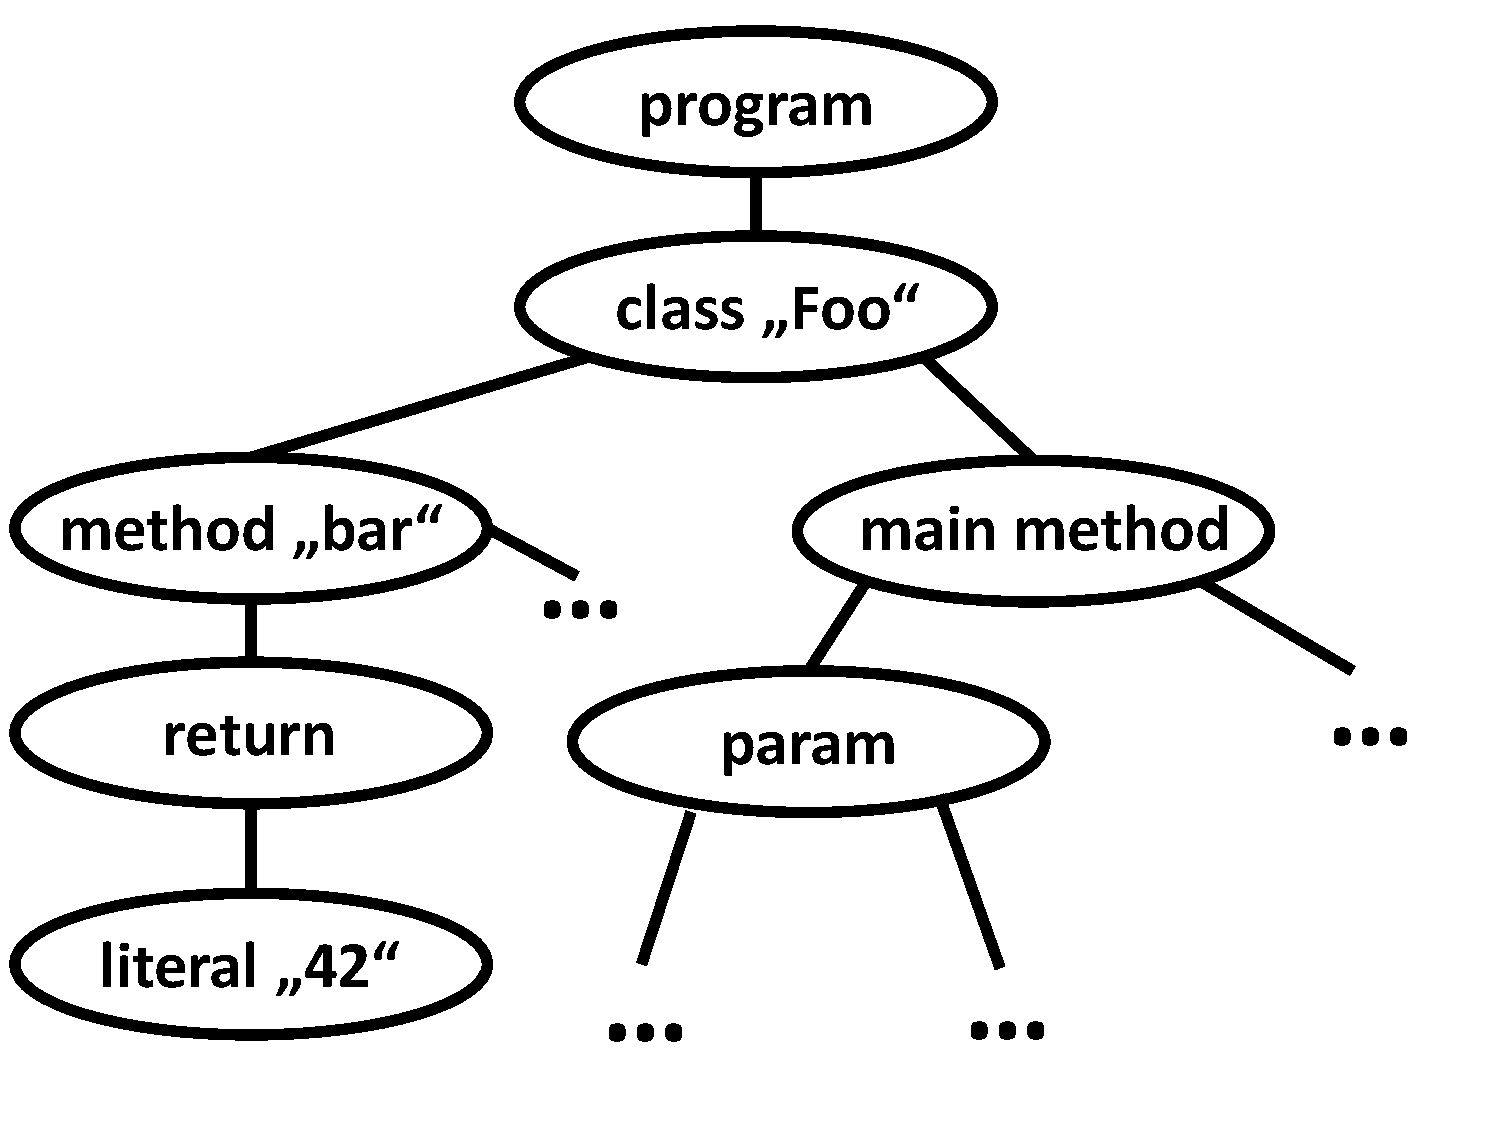
\includegraphics[scale=0.3]{images/AST.pdf}
     \end{center}
\end{frame}